\chapter{روش پیشنهادی}
%\thispagestyle{empty}

\section{مقدمه}

روش‌های موجود در زمینه یادگیری پیوسته برای داده‌های ویدیویی با وجود پیشرفت‌های اخیر، همچنان با مشکلات اساسی روبه‌رو هستند. اغلب این روش‌ها برای مقابله با فراموشی فاجعه‌بار به استفاده از بافرهای بازپخش یا ذخیره‌سازی داده‌های قبلی متکی هستند که نیازمند حافظه بالا و ناسازگار با محدودیت‌های حریم خصوصی است. از طرفی، برخی رویکردها به مدل‌های از پیش آموزش‌دیده متکی‌اند، اما برای انطباق با داده‌های ویدیویی نیاز به آموزش یا تنظیم مجدد کدگذارهای زمانی دارند، که فرآیندی زمان‌بر، پرهزینه و وابسته به منابع سخت‌افزاری سنگین است. علاوه بر این، بسیاری از این روش‌ها از ساختارهای مبتنی بر وظیفه
\LTRfootnote{Task specific}
استفاده می‌کنند که مدیریت و نگهداری آن‌ها در سناریوهای واقعی و وظایف متوالی دشوار بوده و باعث کاهش تعمیم‌پذیری می‌شود.

با توجه به این محدودیت‌ها، نیاز به رویکردهایی احساس می‌شود که بتوانند بدون وابستگی به ذخیره‌سازی وسیع داده‌های گذشته یا آموزش سنگین کدگذارها، عملکرد بهتری در داده‌های ویدیویی ارائه دهند و در عین حال ماهیت مستقل از وظیفه
\LTRfootnote{Task-agnostic}
 داشته باشند. هدف چنین رویکردهایی این است که از ظرفیت مدل‌های بزرگ و از پیش آموزش‌دیده استفاده کرده و با اضافه کردن لایه‌های سبک یا پرامپت‌های یادگیرنده، بدون تغییر مستقیم عامل‌های اصلی مدل، دانش قبلی را حفظ و با داده‌های جدید تطبیق یابند.

در این راستا، ما روشی پیشنهادی ارائه می‌دهیم که با ترکیب قابلیت‌های روش \lr{Open-VCLIP} \cite{open-vclip}و ایده‌های روش \lr{L2P} \cite{l2p}، از پرامپت‌های سبک و پویا برای انطباق با وظایف جدید استفاده می‌کند و نیاز به آموزش سنگین کدگذارهای زمانی را برطرف می‌سازد. این روش با بهره‌گیری بهینه از دانش مدل‌های پیش‌آموزش‌دیده، کاهش فراموشی فاجعه‌بار و حفظ کارایی در سناریوهای واقعی را هدف قرار داده است. انتظار می‌رود این روش با مصرف سخت‌افزاری کمتر، وظایف جدید را به‌طور پیوسته فراگرفته و بدون وابستگی به شناسه وظایف، عملکردی کارآمد و مقیاس‌پذیر ارائه دهد.

\section{روش پیشنهادی برای یادگیری پیوسته تشخیص حرکت انسان}
در این بخش، روش پیشنهادی ما برای یادگیری پیوسته تشخیص حرکت انسان معرفی می‌شود که بر پایه‌ی ترکیب دو رویکرد \lr{Open-VCLIP} و \lr{L2P}، بنا شده است. ایده‌ی اصلی این روش آن است که از قابلیت‌های \lr{Open-VCLIP} برای استخراج ویژگی‌های چندماهیتی (تصویر-متن) بهره گرفته و در عین حال از سازوکار پرامپت‌های یادگیرنده در \lr{L2P} استفاده شود تا مدل بتواند بدون نیاز به تغییر مستقیم عامل‌های کدگذار اصلی، خود را با وظایف متوالی تطبیق دهد. این ترکیب باعث می‌شود که مشکل فراموشی فاجعه‌بار کاهش یافته، حافظه‌ی مورد نیاز برای ذخیره‌سازی نمونه‌ها به حداقل برسد و مدل به صورت مستقل از وظیفه، وظایف جدید را پردازش کند. به عبارت دیگر، ما با این رویکرد سعی کرده‌ایم مزیت‌های هر دو روش را با هم ترکیب کنیم: قدرت تعمیم‌دهی و دانش وسیع \lr{Open-VCLIP} و انعطاف‌پذیری \lr{L2P} در مدیریت وظایف پیوسته. مدل پیشنهادی ما که \lr{ProActionCLIP} 
\RTLfootnote{این نام مخفف \lr{Prompt Action recognition CLIP} 
می‌باشد که به استفاده از روش‌ پرامپت‌گذاری برای تشخیص حرکت توسط مدل کلیپ، اشاره می‌کند.
}
نامگذاری شده است، شامل دو مرحله‌‌ی آموزش  و آزمون می‌باشد که پس از معرفی مدل‌های پایه‌ ی استفاده شده، به توضیح آن‌ها پرداخته می‌شود.
\section{مدل \lr{Open-VCLIP}}
مدل‌های بینایی-زبان مانند \lr{CLIP}، به دلیل توانایی یادگیری نمایش‌های مشترک تصویر و متن، عملکرد قابل توجهی در وظایف بینایی و زبانی داشته‌اند. با این حال، این مدل‌ها در حالت پایه برای داده‌های ایستا (تصاویر) طراحی شده‌اند. \lr{Open-VCLIP} با گسترش معماری \lr{CLIP} و افزودن قابلیت درک اطلاعات زمانی، این محدودیت را برطرف می‌کند و روشی کارآمد برای تحلیل ویدیو و یادگیری مستمر ارائه می‌دهد که در ادامه آن را بررسی می‌کنیم. 
\subsection{تبدیل \lr{CLIP} مبتنی بر تصویر به \lr{CLIP} مبتنی بر ویدیو}
در این بخش، ورودی ویدیویی به دنباله‌ای از فریم‌ها تبدیل می‌شود و هر فریم توسط کدگذار تصویری \lr{CLIP} به یک بردار ویژگی تبدیل می‌گردد. سپس این ویژگی‌ها در قالب دنباله‌ای زمانی قرار گرفته و با سازوکار توجه ترکیب می‌شوند. در سازوکار توجه فرمول محاسبه‌ی خروجی مطابق \eqref{eq:attention_basic} می‌باشد.
\begin{equation}\label{eq:attention_basic}
	y_{s,t} = \mathrm{Softmax}\left( \frac{q_{s,t} K_{t}^{\mathrm{T}}}{\sqrt{d}} \right) V_{t},
\end{equation}
در این رابطه، $q_{s,t}$ بردار پرسمان \LTRfootnote{Query} برای یک وصله
	\LTRfootnote{Patch}
	 از تصویر، $K_t$ ماتریس کلید و $V_t$ ماتریس مقدار برای قاب یا تصویر $t$ هستند که از طریق سازوکار توجه ترکیب می‌شوند. در این حالت، ارتباط یک وصله از تصویر با خودش و بقیه‌ی وصله‌های تصویر مشخص می‌شود. برای سازگار کردن مدل برای ویدیو در مدل \lr{Open-VCLIP}، بردار پرسمان وصله‌ی قاب فعلی را در ماتریس کلید قاب فعلی، بعدی و قبلی ضرب می‌کند و پس از اجرای تابع \lr{softmax} نیز در ماتریس مقدار قاب فعلی، بعدی و قبلی ضرب می‌کند و سازوکار توجه را مانند \eqref{eq:attention_extended}، محاسبه می‌کند. در این صورت نه تنها ارتباط وصله‌ی قاب فعلی با قاب خودش، بلکه با قاب قبلی و بعدی خود نیز در نظر گرفته می‌شود. این راهکار به ظاهر ساده، توانست تحول خوبی در زمینه‌ی سازگاری مدل \lr{CLIP} با داده‌ی ویدیویی ایجاد کند.
\begin{equation}\label{eq:attention_extended}
	y_{s,t} = \mathrm{Softmax}\left( 
	\frac{q_{s,t} \left[ K_{(t-1)\sim(t+1)} \right]^{\mathrm{T}}}{\sqrt{d}} 
	\right) 
	\left[ V_{(t-1)\sim(t+1)} \right],
\end{equation}

‌\begin{figure}
	\centering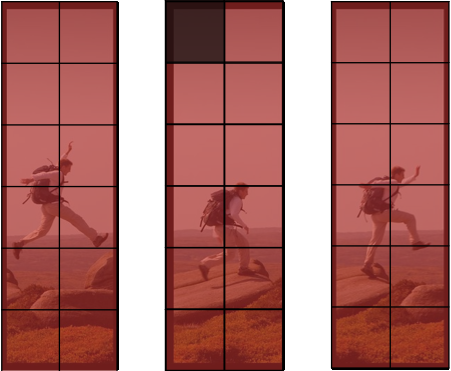
\includegraphics[scale=.50]{Images/Chapter3/openvclip_attention.png}
	\caption[]{ وصله‌های درنظر گرفته شده برای هر وصله از قاب در سازوکار تغییر یافته‌ی توجه}
	\label{fig.31}
\end{figure}




\subsection{منظم‌سازی وزن‌های میان‌یابی}
برای جلوگیری از فراموشی دانش پیش‌آموزش و در عین حال سازگار کردن مدل با داده‌های جدید، منظم‌سازی وزن‌های میان‌یابی
\LTRfootnote{Interpolation Weight Regularization (IWR)}
 معرفی شده است. در این روش، وزن‌های مدل به‌صورت ترکیبی از عامل‌های اولیه (پیش‌آموزش) و عامل‌های به‌روزرسانی‌شده در وظیفه جدید، تنظیم می‌شوند. این میان‌یابی به مدل کمک می‌کند تا در حین یادگیری، تعادلی میان دانش قدیمی و اطلاعات تازه برقرار کرده و از بیش‌برازش
 \LTRfootnote{Overfitting}
  جلوگیری کند.
\section{مدل \lr{L2P}}
\section{مرحله‌ی آموزش}
همانطور که پیش‌تر اشاره شد، در مرحله‌ی آموزش، تمرکز بر یادگیری پرامپت‌های مناسب برای دسته‌های مختلفی است که به صورت پیوسته به مدل اضافه می‌شوند. طرح کلی مدل در مرحله‌ی آموزش در \cref{fig.31}، نشان داده شده است.

‌\begin{figure}
	\centering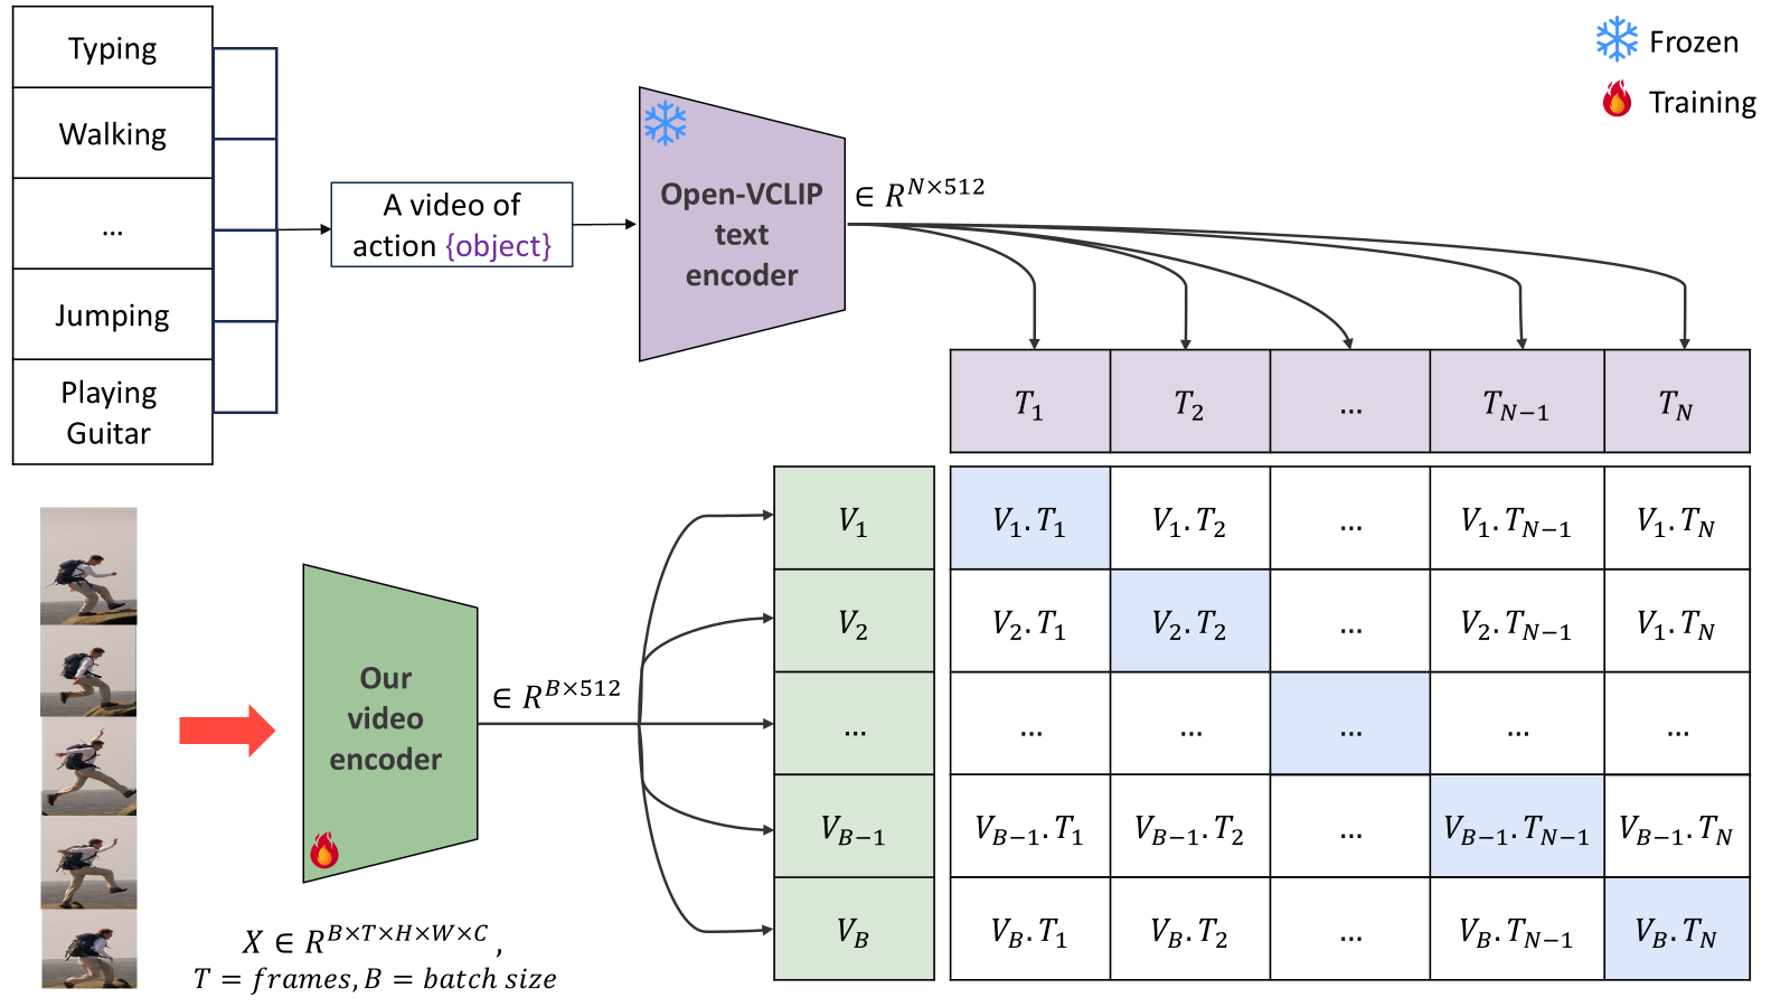
\includegraphics[scale=.50]{Images/Chapter3/train_phase.png}
	\caption[]{طرح کلی مرحله‌ی آموزش مدل \lr{ProActionCLIP}}
	\label{fig.31}
\end{figure}

\section{رعایت قواعد نشانه‌گذاری}
منظور از نشانه‌گذاري به‌کار‌بردن علامت‌ها و نشانه‌هايي است که خواندن و فهم درست یک جمله را ممکن و آسان مي‌کند. در ادامه نشانه‌هاي معمول و متداول در زبان فارسي و موارد کاربرد آنها به اختصار معرفی می‌شوند.

\subsection{ويرگول}
ويرگول نشانه ضرورت یک مکث کوتاه است و در موارد زير به‌کار مي‌رود:
\begin{itemize}
\item
در ميان دو کلمه که احتمال داده شود خواننده آنها را با کسره اضافه بخواند، يا نبودن ويرگول موجب بروز اشتباه در خواندن جمله شود.
\item
در موردي که کلمه يا عبارتي به‌‌‌‌عنوان توضيح، در ضمن یک جمله آورده شود. مثلاً برای کنترل وضعیت فضاپیماها، به‌دلیل آن‌که در خارج از جو هستند، نمی‌توان از بالک‌های آیرودینامیکی استفاده کرد.
\item
جدا‌کردن بخش‌هاي مختلف يک نشاني يا یک مرجع
\item
موارد دیگر از این قبیل
\end{itemize}
پیش از ويرگول نبايد فاصله گذاشته شود و پس از آن يک فاصله لازم است و بيشتر از آن صحیح نیست.
\subsection{نقطه}
نقطه نشانه پایان یک جمله است. پیش از نقطه نبايد فاصله گذاشته شود و پس از آن يک فاصله لازم است و بيشتر از آن صحیح نیست.
\subsection{دونقطه}
موارد کاربرد دونقطه عبارتند از:
\begin{itemize}
\item
پيش از نقل قول مستقيم
\item
پيش از بيان تفصيل مطلبي که به اجمال به آن اشاره شده‌است.
\item
پس از واژه‌اي که معني آن در برابرش آورده و نوشته مي‌شود.
\item
پس از کلمات تفسير‌کننده از قبيل «يعني» و ...
\end{itemize}
پیش از دونقطه نبايد فاصله گذاشته شود و پس از آن يک فاصله لازم است و بيشتر از آن صحیح نیست.
\subsection{گیومه}
موارد کاربرد گیومه عبارتند از:
\begin{itemize}
\item
وقتي که عين گفته يا نوشته کسي را در ضمن نوشته و مطلب خود مي‌آوريم. 
\item
در آغاز و پايان کلمات و اصطلاحات علمي و يا هر کلمه و عبارتي که بايد به‌صورت ممتاز از قسمت‌هاي ديگر نشان داده شود.
\item
در ذکر عنوان مقاله‌ها، رساله‌ها، اشعار، روزنامه‌ها و ...
\end{itemize}
\subsection{نشانه پرسشی}
پیش از «؟» نبايد فاصله گذاشته شود و پس از آن يک فاصله لازم است و بيشتر از آن صحیح نیست.
\subsection{خط تیره}
موارد کاربرد خط تیره عبارتند از:
\begin{itemize}
\item
جدا‌کردن عبارت‌هاي توضيحي، بدل، عطف بيان و ...
\item
به‌جاي حرف اضافه «تا» و «به» بين تاريخ‌ها، اعداد و کلمات
\end{itemize}
\subsection{پرانتز}
موارد کاربرد پرانتز عبارتند از:
\begin{itemize}
\item
به‌معني «يا» و «يعني» و وقتي که یک کلمه يا عبارت را براي توضيح بيشتر کلام بياورند.
\item
وقتي که نويسنده بخواهد آگاهي‌هاي بيشتر (اطلاعات تکميلي) به خواننده عرضه کند.
\item
براي ذکر مرجع در پايان مثال‌ها و شواهد.
\end{itemize}
نکته: بین کلمه یا عبارت داخل پرانتز و پرانتز باز و بسته نباید فاصله وجود داشته باشد.
\section{جدا یا سرهم نوشتن برخی کلمات}
تقريباً تمامي کلمات مرکب در زبان فارسي بايد از هم جدا نوشته شوند؛ به استثناي صفات فاعلي مانند «عملگر»، «باغبان» و يا «دانشمند» و کلماتي نظير «اينکه»، «آنها». در ادامه به نمونه‌هايي از مواردي که بايد اجزاي يک کلمه جدا، اما بدون فاصله نوشته شوند، اشاره مي‌شود‌:
\begin{enumerate}
\item
در افعال مضارع و ماضی استمراری که با «می» شروع می‌شوند، لازم است که در عين جدا نوشتن، «می» از بخش بعدي فعل جدا نيافتد‌.‌ برای اين منظور بايد از «فاصله متصل» استفاده و «می» در اول فعل با \lr{SS}\LTRfootnote{Shift+Ctrl+@} از آن جدا شود.‌ به‌طور مثال «می‌شود» به‌جاي «می شود». 
\item
	«ها»ی جمع بايد از کلمه جمع بسته‌شده جدا نوشته شود؛ مگر در برخی کلمات مانند «آنها». اين امر در مورد کلمات غير‌فارسي که وارد زبان فارسي شده‌اند و با حرف «ها» جمع بسته می‌شوند، مانند «کانال‌ها» يا «فرمول‌ها» مورد تاکيد است.
\item
	حروف اضافه مانند «به» وقتي به‌صورت ترکيب ثابت همراه کلمه پس از خود آورده می‌شوند، بهتر است با \lr{SS} از آن جدا شوند‌.‌ مانند «به‌صورت»، «به‌عنوان» و «به‌‌‌لحاظ»‌.‌ لازم به ذکر است هنگامی که حرف اضافه «به» با کلمه پس از خود معناي قيدي داشته باشد، مثل «بشدت» يا «بسادگي»، بهتر است که به‌صورت چسبيده نوشته شود‌.
\item
	کلمات فارسی نبايد با قواعد عربی جمع بسته شوند؛ پس «پيشنهادها» صحيح و «پيشنهادات» اشتباه است‌.‌
\item
	اسم‌ها و صفت‌هاي دو‌قسمتي مثل «خط‌چين» و «نوشته‌شده» با \lr{SS} از هم جدا می‌شود‌.‌
\item
	شناسه‌ها با \lr{SS} از کلمه اصلي جدا می‌شود‌.‌ مثل «شده‌اند»‌ و «شده‌است». 
\item
	‌ «است» هنگامی که نقش شناسه را داشته باشد توسط \lr{SS} از قسمت اصلي جدا می‌شود‌.‌ مانند «گفته‌است»‌.
\item
	بند پیشین نبايد باعث افراط در استفاده از فاصله متصل شود. مثلاً عبارت «نوشته می‌شود‌« صحيح و عبارت «نوشته‌می‌شود» ناصحیح است. 
\item
	فعل‌هاي دو‌کلمه‌اي که معناي اجزاي آنها کاملاً با معناي کل متفاوت است، بهتر است که با \lr{SS} از هم جدا ‌شوند‌.‌
\item
	کلمات مرکب مثل کلمه «دوکلمه‌اي» در عبارت «فعل‌هاي دوکلمه‌اي» و «يادداشت‌برداري».
\item
	مصدرهاي دو قسمتي با \lr{SS} از هم جدا می‌شوند‌.‌ مثل «ذوب‌کردن» و «واردکردن»‌.
\item
	 صفات تفضيلي مثل « آسان‌تر».
\end{enumerate}

